\documentclass[12pt]{amsart} 

\usepackage{blindtext}
\usepackage[utf8]{inputenc}
\usepackage[american]{babel}

\usepackage{csquotes}
\usepackage[style=numeric,
    citestyle=numeric,
    backend=biber,
    natbib=true,
url=true]{biblatex}

\usepackage[hidelinks]{hyperref}
\usepackage{setspace}
\usepackage{microtype}

\bibliography{main.bib}

\usepackage[margin=1in]{geometry}
\usepackage{graphicx}
\usepackage{fancyhdr}
\usepackage{lastpage}
\pagestyle{fancy}
\renewcommand{\headrulewidth}{0.0pt}

\lhead{Team \# 54040}
\rhead{Page \thepage\ of \pageref{LastPage}}
\cfoot{}

\usepackage{amsmath, amssymb, amsthm}
\usepackage{ragged2e}

% Custom macros
\newcommand{\la}{\overleftarrow}
\newcommand{\ra}{\overrightarrow}
\newcommand{\ca}{\overleftrightarrow}
\newcommand{\R}{\mathbb{R}}
\newcommand{\abs}[1]{\left|#1\right|}
\DeclareMathOperator*{\argmin}{\mathrm{arg\,min}}

\title{Keeping it even: maintaining evenly distributed temperatures within a
two-dimensional bathtub}

\date{February 1, 2016}

\begin{document}

\maketitle

\thispagestyle{fancy}
\tableofcontents

\begin{abstract}

\end{abstract}

\section{Introduction}

The avid bather faces the constant struggle in balancing her ability to relax in
the bathtub and in keeping an evenly distributed water temperature within the
tub. For such a bather a quality bath is a necessity. Necessity, the mother of
invention, requires that quality be sought after and maximized---the bather
should need to worry as little as possible about the quality of the temperature
distribution in the tub. To help our bather, we seek to give a precise
determination of quality and pose a question in whose answer provides the best
such quality. Yet living in a world of scarce resources demands attention
towards the cost of our decisions. Our underlying quest for quality needs
temperament from reality, and we shall formulate the problem as a trade-off
between these competing camps.

In this work, we begin by developing a model for the evolution of heat in a
bathtub. Heat travels through a fluid by two means: diffusion and convection.
The diffusion process refers to the natural spread of heat from high-temperature
peaks to low-temperature valleys. This process is fundamentally spatial and
occurs even in the context of a stationary fluid. The convection process, by
contrast, refers to the spread of heat subject to a moving fluid. Heat can flow
with a fluid to spread along the direction the fluid travels; this process helps
to explain the behavior of ocean conveyor belts and hurricanes. In order to
optimize the distribution of heat, we need to understand how heat evolves. This
will be the primary scope of our paper.

Our work proceeds as follow. Section 2 describes the high-level view of the
computational model for simulating the evolution of heat in a bathtub in the
context of both a stationary and moving fluid. It also outlines the numerical
methods we will use in order to approximate the underlying diffusion and
convection processes. We also propose, but do not solve, the bather's
optimization problem. Section 3 provides the results of our initial 


\section{Model overview}

Throughout this work we will denote the spatial region under scrutiny by
$\Omega \subseteq \R^2$, and we write $\partial \Omega$ to indicate the
boundary of the region. The function $T : \Omega \times \R_{\geq 0} \to \R$
will denote the temperature $T = T(x,y,t)$, and the functions $v_x : \Omega
\times \R_{\geq 0} \to \R$ and $v_y : \Omega \times \R_{\geq 0} \to \R$ will
denote $v_x = v_x(x,y,t)$ the horizontal and $v_y = v_y(x,y,t)$ the vertical
components of the velocity of the fluid flow. 

\subsection{Two-dimensional Navier-Stokes formulation}

The Navier-Stokes equations for an incompressible fluid are given by
\begin{align}
    \nabla \cdot v &= 0 \\
    \frac{\partial v}{\partial t} + (v \cdot \nabla) v &= -
    \frac{1}{\rho} \nabla p + \alpha \nabla^2 v
    \label{eq:\theequation}
\end{align}
where $v = (v_x, v_y)$ is the fluid velocity, $\rho$ denotes mass density of
the fluid, and $p$ denotes pressure. Incompressibility is incorporated
through Equation (), since nonzero divergence implies the presence of either
sources or sinks of fluid. Now because $v$ is two-dimensional, Equation
() actually implies a pair of partial differential equations for both the $x$
and $y$ components. The pressure $p$ is determined through the Poisson equation
\begin{equation}
    \nabla^2 p = b,
    \label{eq:\theequation}
\end{equation}
where $b$ is taken as a constant term for the purposes of this study. Many
wonderful resources exist online for understanding the formulation of these
equations, specifically Barba's work \cite{12-steps}, but we do not include a
derivation of these relations here.

\subsection{Heat convection-diffusion equation}

The heat convection-diffusion equation found in the literature
\cite{convection-diffusion},
\begin{equation}
    \frac{\partial T}{\partial t} - \alpha \nabla^2 T + v \cdot \nabla T =
    0,
    \label{eq:\theequation}
\end{equation}
is a combination of parabolic and hyperbolic partial differential equations
relating the temporal change in temperature with its spatial diffusion and
the flow of heat packets elsewhere in the fluid.     Here, $\nabla$ is the
gradient operator $\left( \frac{\partial}{\partial x},
\frac{\partial}{\partial y} \right)$, $\nabla^2$ denotes the Laplacian
$\frac{\partial^2}{\partial x^2} + \frac{\partial^2}{\partial y^2}$, $v =
(v_x, v_y)$ denotes the fluid velocity vector, and $\alpha$ is a diffusivity
constant.

The ubiquity of parabolic PDEs in modeling scientific phenomenon is well
known, since it captures the essence of diffusive processes. Elliptic PDEs
often arise out of physical environments with a present potential field
(e.g.  gravitational or electrostatic), or in the cases of incompressible
fluid flow \cite{convection-diffusion, ames}. We use the latter for
motivating this model, as bathtub water exhibits the standard
characteristics of incompressible fluid.

\subsection{Numerical methods}

We proceed by providing a brief overview of the numerical methods used in
this study. To approximate the solution to a PDE, we discretize the region
$\Omega$ under consideration into a coordinate mesh. For convention, we
write $T_{i,j}^{n}$ to denote the temperature at the $(i,j)$ mesh coordinate
at the time interval $t=n$. 

Modifying the notation employed by Ames \cite{ames}, we establish the
following nomenclature for the numerical operations in the model (the use of $T$
is without loss of generality and can be substituted for $v$ and $p$ as well):

\begin{center}
    \begin{tabular}[]{ll}
        $\ra{\Delta_i} T_{i,j}^n = T_{i+1,j}^n - T_{i,j}^n$ & Forward
        differencing \\
        $\la{\Delta_i} T_{i,j}^n = T_{i,j}^n - T_{i-1,j}^n$ & Backward differencing \\
        $\ca{\Delta_i} T_{i,j}^n = T_{i+1/2,j}^n - T_{i-1/2,j}^n$ & Central differencing
    \end{tabular}
\end{center}

The estimation of partial derivatives using the above techniques result in
different rates of convergence as the numerical increment decreases. In
particular, we have
\begin{equation}
    \frac{\partial T_{i,j}^n}{\partial x} = \frac{\ra{\Delta_j}T_{i,j}^n}{\Delta
    x}+ O(\Delta x),
    \label{eq:\theequation}
\end{equation}
(while we use differentiation along the horizontal axis, the
convergence is without loss of generality of axis), and we similarly have
\begin{equation}
    \frac{\partial T_{i,j}^n}{\partial x} = \frac{\la{\Delta_j}T_{i,j}^n}{\Delta
    x} + O(\Delta x),
    \label{eq:\theequation}
\end{equation}
while for central differencing, we have
\begin{equation}
     \frac{\partial T_{i,j}^n}{\partial x} = \frac{\ca{\Delta_j}T_{i,j}^n}{\Delta
    x} + O((\Delta x)^2).
    \label{eq:\theequation}
\end{equation}
Indeed, as $\Delta x \to 0$ we see that central differencing has a quadratic
rate of convergence, while forward and backward differencing are linear. For
this advantage we employ central differencing in computing spatial derivatives.
However, as the time evolution is simulated on the fly, we cannot have access to
$T_{i,j}^{n+1}$ when computing $T_{i,j}^n$. We consequently use backward
differencing to estimate the time derivative.

The approximated Navier-Stokes equations now read
\begin{align}
    \frac{\ca{\Delta_{j}}(v_x)_{i,j}^n}{\Delta x} +
    \frac{\ca{\Delta_{i}}(v_y)_{i,j}^n}{\Delta y} &= 0 \\
    \frac{\la{\Delta_n}v^{n}_{i,j}}{\Delta t} + (v_x)_{i,j}^{n}
    \frac{\ca{\Delta_{j}}(v_x)_{i,j}^n}{\Delta x} + (v_y)_{i,j}^n
    \frac{\ca{\Delta_{i}}(v_y)_{i,j}^n}{\Delta y} &=
    -\frac{1}{\rho} \left(  \frac{\ca{\Delta_j}p_{i,j}^n}{\Delta
    x}+\frac{\ca{\Delta_i}p_{i,j}^n}{\Delta y}  \right) + \alpha
    \left(\frac{\ca{\Delta_{j}}^2(v_x)_{i,j}^n}{(\Delta x)^2} + 
    \frac{\ca{\Delta_{i}}^2(v_y)_{i,j}^n}{(\Delta y)^2}
    \right).
\end{align}
The Poisson equation is 
\begin{equation}
    \frac{\ca{\Delta_{j}}^2p_{i,j}^n}{(\Delta x)^2} + 
    \frac{\ca{\Delta_{i}}^2p_{i,j}^n}{(\Delta y)^2}
    = b.
    \label{eq:\theequation}
\end{equation}
Finally, heat convection-diffusion is given by
\begin{equation}
    \frac{\la{\Delta_n}T_{i,j}^n}{\Delta t} - \alpha \frac{\ca{\Delta_{j}}^2T_{i,j}^n}{(\Delta x)^2} + 
    \frac{\ca{\Delta_{i}}^2T_{i,j}^n}{(\Delta y)^2} + (v_x)_{i,j}^n
    \frac{\ca{\Delta_{j}}T_{i,j}^n}{\Delta x} + (v_y)_{i,j}^n
    \frac{\ca{\Delta_{i}}T_{i,j}^n}{\Delta y} = 0
    \label{eq:\theequation}
\end{equation}

The algorithmic approach we take is as follows. Using the numerical formulas
given above, isolate the time derivative and set its value to the other side of
the equation. In the case of temperature, for example, we then update its value
with
\begin{equation}
    T_{i,j}^{n+1} \leftarrow T_{i,j}^{n} + \Delta t \cdot \frac{\partial
        T_{i,j}^n}{\partial t}.
    \label{eq:\theequation}
\end{equation}
This pattern is used throughout the computer implementation of these models. The
remaining question is the stability of these results. In fact, as we shall
discuss in Section 4, these equations can be highly unstable, especially with a
naive assignment of parameter values.



\subsection{Bathtub optimization problem}

The goal of this study is to identify a process through which the avid bather
may seek to achieve uniform water temperature, ideally wasting as little water
as possible. Using the aforementioned numerical models to simulate bathtub
dynamics, we propose an optimization problem by which to approach this goal. Let
$t_{\mathrm{total}}$ indicate the period in which the faucet is turned on, let
$T_{\mathrm{f}}$ denote the temperature of the water in the faucet, and let
$V(t)$ denote the total volume of water that has left the faucet. We assume that
$\frac{dV}{dt} = c$, i.e., the strength of the faucet is fixed at a chosen $c$ throughout the
duration of the bath. Now, consider the surface integral
\begin{equation}
    f_{\mathrm{cont}}(t) = \int_{\Omega} \abs{T(x,y,t) - T_{\mathrm{f}}} \ d\omega.
    \label{eq:\theequation}
\end{equation}
We propose the minimization problem
\begin{equation}
    \argmin_{c} \int_{0}^{t_{\mathrm{total}}} V(t) \ dt \quad \text{such that}
    \quad \int_{0}^{t_{\mathrm{total}}} f_{\mathrm{cont}}(t) \ dt < \gamma,
    \label{eq:\theequation}
\end{equation}
where $\gamma$ is some tolerance for variation. This is minimization
problem is subject to a total variation constraint, which has been subject to
considerable study, especially within the context of medical imaging
\cite{Zhang2005}.

This optimization leads to a natural discretization. We rewrite:
\begin{align}
    V(t) &\longrightarrow V^t \\
    \frac{dV}{dt} = c &\longrightarrow V^{t+1} - V^t = c \\
    f_{\mathrm{cont}}(t) = \int_{\Omega} \abs{T(x,y,t) - T_{\mathrm{f}}} \
    d\omega &\longrightarrow f_{\mathrm{disc}}(t) = \sum_{x,y}\abs{T(x,y,t) -
        T_{\mathrm{f}}},
\end{align}
which translate to the problem
\begin{equation}
    \argmin_{c} \sum_{t=0}^{t_{\mathrm{total}}}V^{t_{\mathrm{total}}} \quad \text{such that} \quad
    \sum_{t=0}^{t_{\mathrm{total}}} f_{\mathrm{disc}}(t) < \gamma.
    \label{eq:\theequation}
\end{equation}

The minimization problem posed here captures the major features of the bathtub
optimizer problem. In our problem, the bather need not frequently calibrate the
settings of the bathtub; rather, the bathtub ``policy'' reduces to an initial
choice of $c$. Moreover, the underlying objective is not to get an even temperature
distribution (as the bather may simply leave the faucet on arbitrarily long to
achieve this), but to conserve as much water as possible. The temperature
distribution problem, then, must be seen within the framework of water
conservation first and not vice versa. On the other hand, the best volume
minimization policy is $c=0$, so the bounded temperature total variation
constraint incorporates the desired $c > 0$ aspects of the problem. Finally,
from both a numerical perspective and a feasibility perspective, demanding
complete temperature uniformity, $\gamma = 0$, is impossible. Instead, $\gamma$
represents the degree of tolerance to which the bather can expect a range of
temperatures in the bathtub.

\section{Empirical results}

Our work is highly preliminary and requires more study in order to better
calibrate our models and properly run experiments. However, we simulated a
number of variously parametrized situations and can report on the model as a
proof of concept.

\subsection{Heat diffusion in a stationary fluid}

\begin{center}
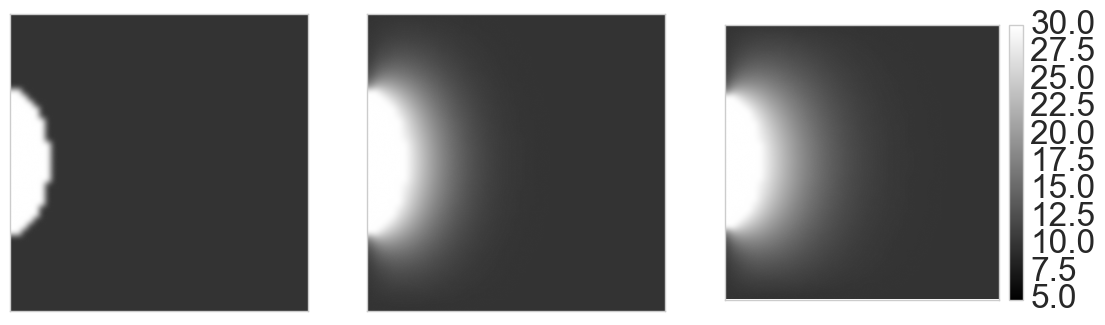
\includegraphics[width=0.8\textwidth]{../plots/diffusion-01.png}

\justify
\footnotesize{
Figure 1: The heat diffusion process in the case of a stationary fluid and
constant faucet tap. The mesh
dimensions are $50 \times 50$, $\alpha = 10^{-3}$, $T_{\mathrm{tub}} = 10$, and
$T_{\mathrm{faucet}} = 30$.}
\end{center}

For example, the above figure shows a heat-diffusion process on a stationary
fluid. The white ellipsoid in the left side of the image represents temperature
emanating from the faucet source. Since the faucet water temperature is greater
than the rest of the bathtub water, we observe temperature diffusion across the
bathtub over time.

The same configuration yields a decreasing total variation of temperature as a function
of time, which corroborates with the intuition that heat diffusing from a source
increases the uniformity of the bathtub heat.

\begin{center}
    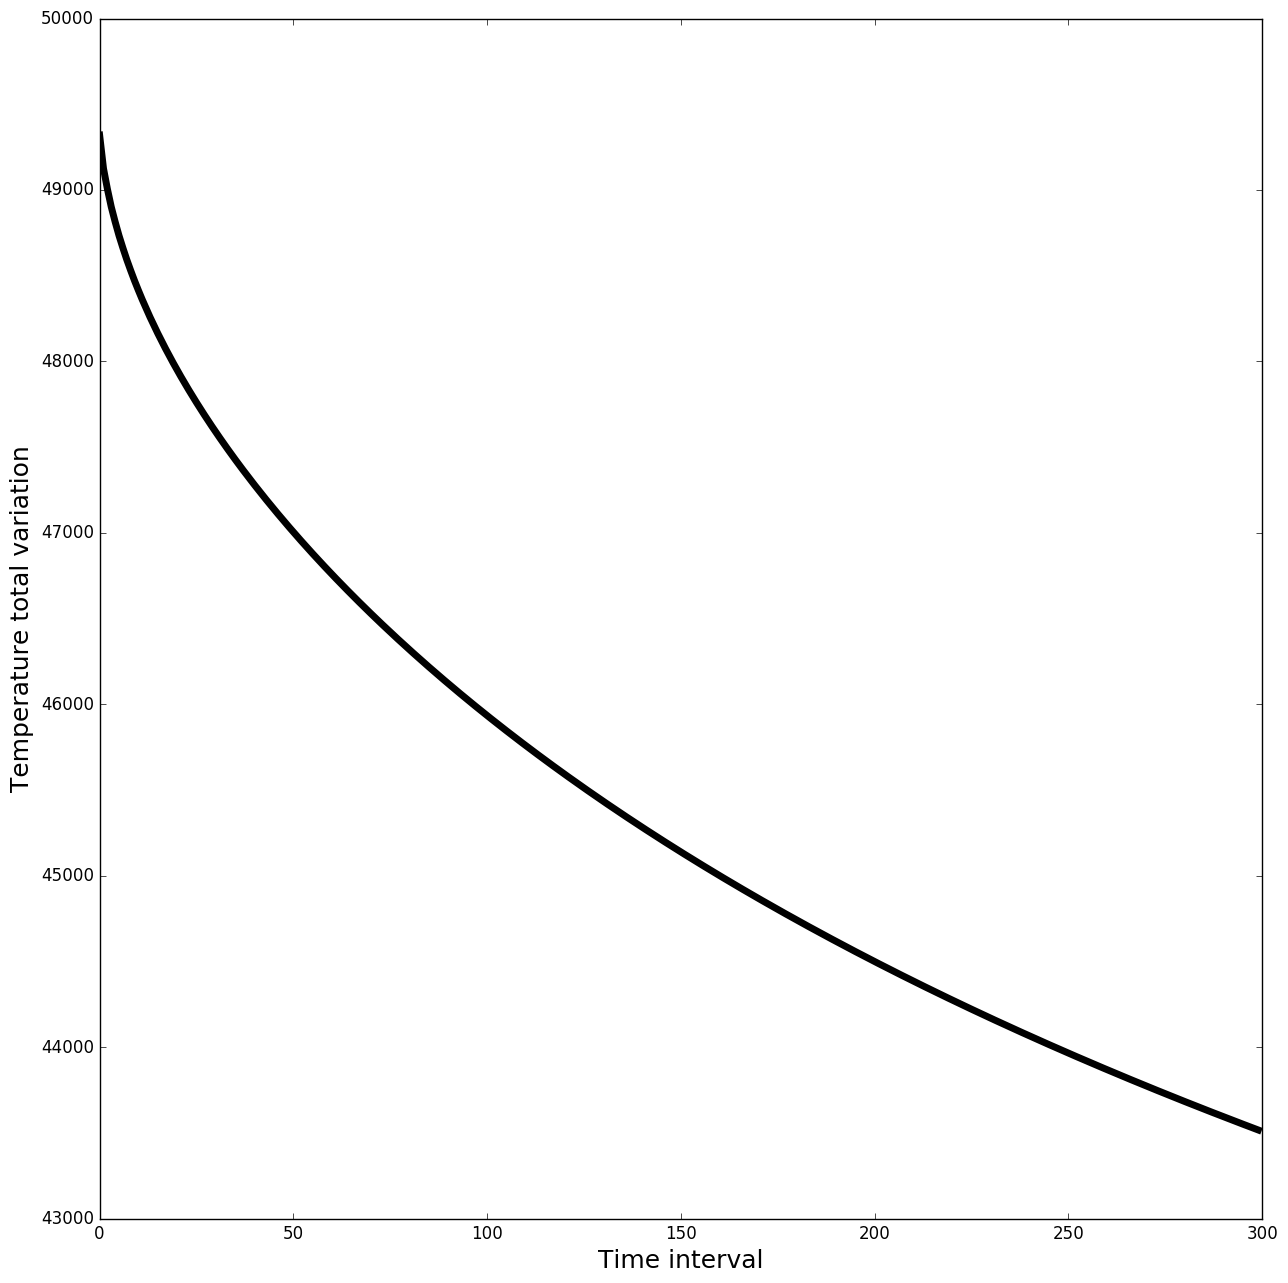
\includegraphics[width=0.5\textwidth]{../plots/tv-01.png}

    \justify
    \footnotesize{
    Figure 2: Temperature total variation over time in the case of a stationary
    fluid, with the same parameters as in Figure 1. The monotonicity of the TV
function is in line with basic intution.}
\end{center}

We can also examine the case in which the faucet water is turned on only for the
initial instant. Our proposed optimization model omits this possibility since it
requires a fixed water flux from the faucet. However, when we formulated the
model we relied on the intuitive justification that the overall temperature
would diverge from the faucet temperature. We simulate the heat diffusion in a
stationary fluid for which the ``faucet'' turns off immediately after the outset
of the simulation. 

\begin{center}
    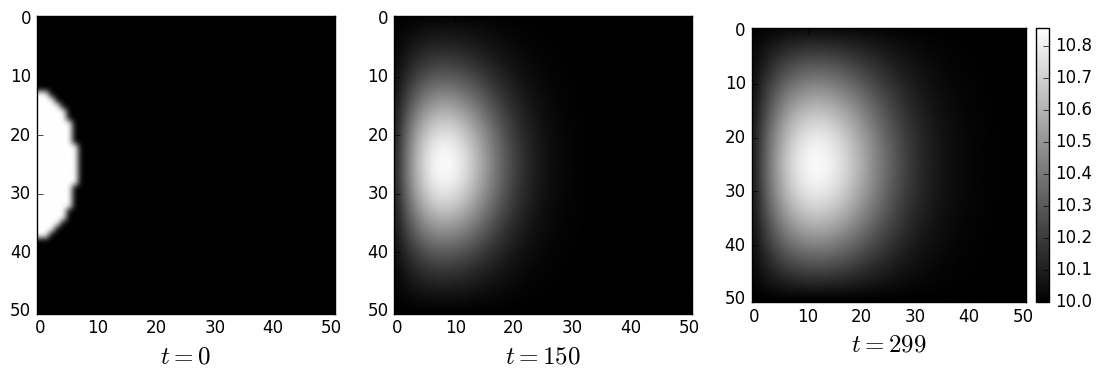
\includegraphics[width=0.8\textwidth]{../plots/diffusion-02.png}

    \justify
    \footnotesize{
    Figure 3: The heat diffusion process in the case of a stationary fluid and
    temporary faucet tap. The mesh dimensions are $50 \times 50$, $\alpha =
    10^{-3}$, $T_{\mathrm{tub}} = 10$, and $T_{\mathrm{faucet}} = 30$.}
\end{center}

We see the overall temperature level decreases rapidly after the first time
interval, but the uniformity increases.  However, as we modeled total variation
as deviation from the faucet temperature, we see that the total variation
receives a higher penalty than before.

\begin{center}
    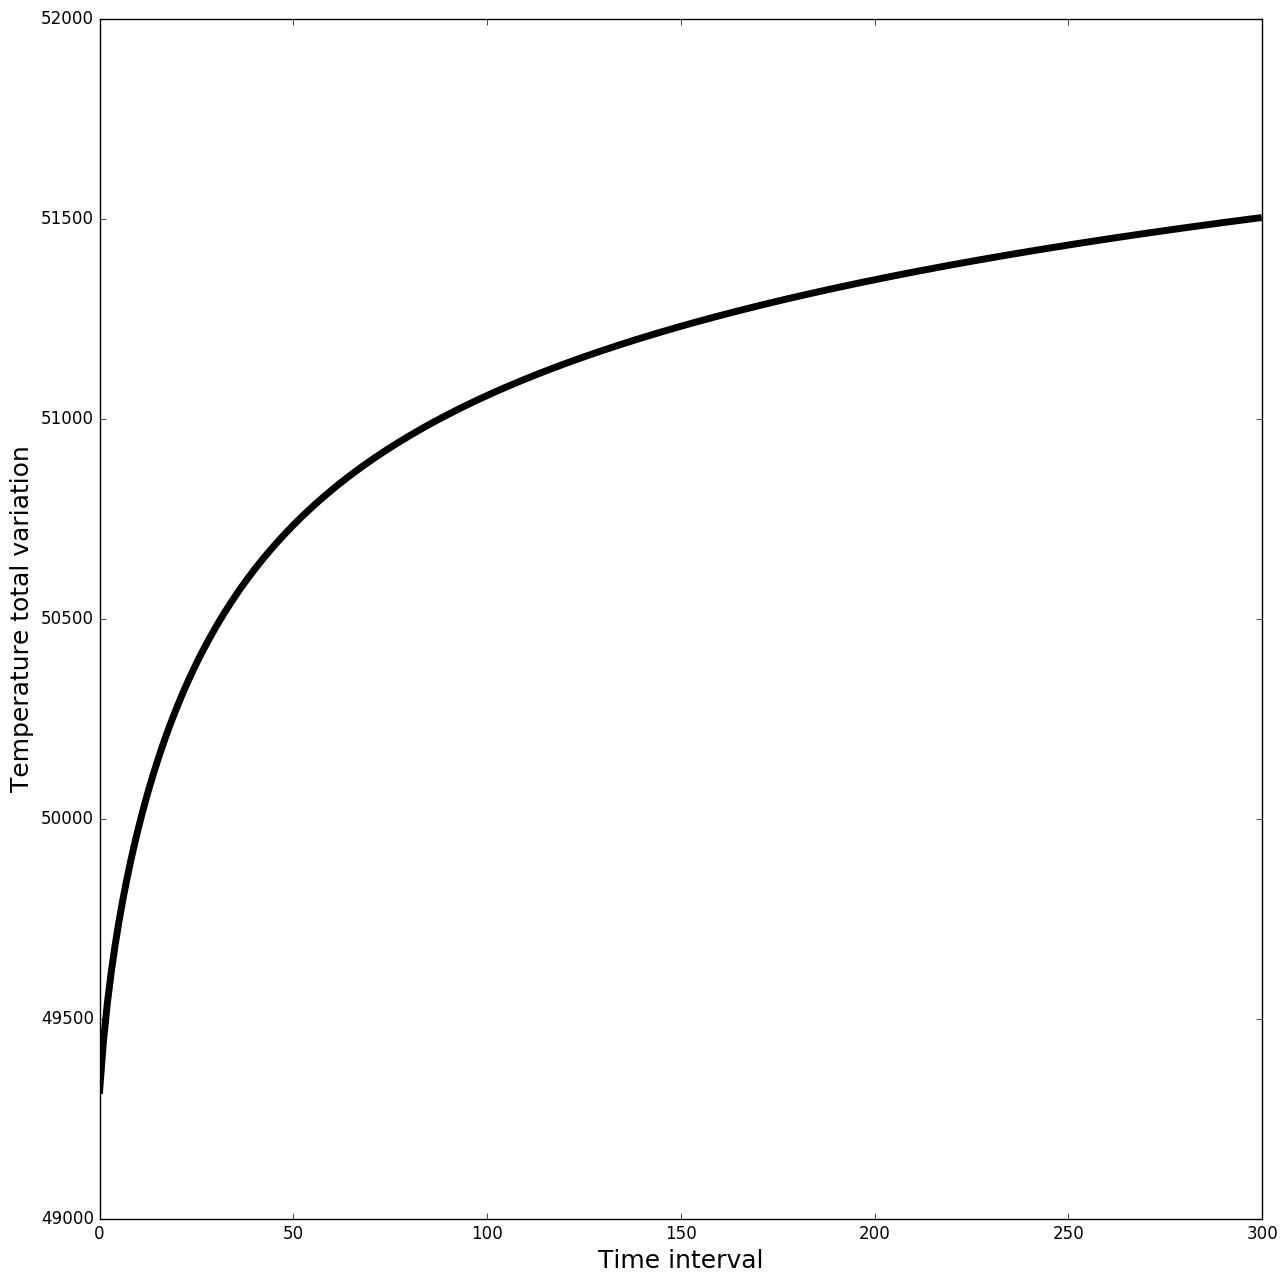
\includegraphics[width=0.5\textwidth]{../plots/tv-02.png}

    \justify
    \footnotesize{
    Figure 4: Temperature total variation over time in the case of a stationary
    fluid, with the same parameters as in Figure 3. The monotonicity of the TV
function is in line with basic intution.}
\end{center}
The fact that the total variation performs so poorly in this case has
implications for the policy problem, which we will discuss in the next section.

\subsection{Nonstationarity and numerical stability}

Generalizing beyond stationary fluids reveals a number of critical issues of the
numerical techniques employed in this study, but also provides useful
information regarding the underlying problem. In stationary fluid, the
Navier-Stokes and Poisson equations are not in play; however, by relaxing the
stationarity constraint, we observe the effects fluid flow on the diffusivity of
heat. We simulate the case described in Figure 1 but relax the stationarity constraint.

\begin{center}
    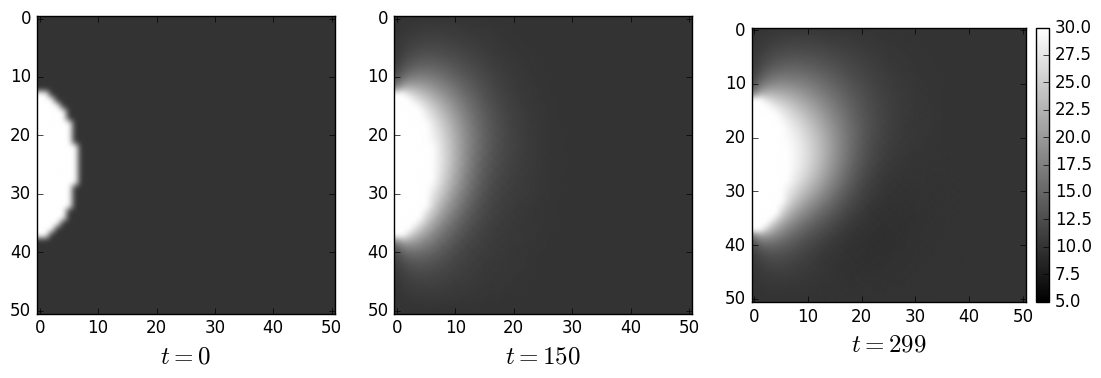
\includegraphics[width=0.8\textwidth]{../plots/diffusion-03.png}

    \justify
    \footnotesize{
    Figure 5: The heat diffusion process in the case of a moving fluid and
    permanent faucet tap. The mesh dimensions are $50 \times 50$, $\alpha =
    10^{-3}$, $T_{\mathrm{tub}} = 10$, and $T_{\mathrm{faucet}} = 30$. The
parameter controlling the fluid motion is set $b = 5$.}
\end{center}

By comparing Figure 5 with Figure 1, we see that adding the convection process
into the model actually improves the spread of the faucet temperature. Since
more of the bathtub area is white in the images, we have more of the surface
area heated by the temperature water. This phenomenon is confirmed by measuring
the total variation of the bathtub water over time.

\begin{center}
    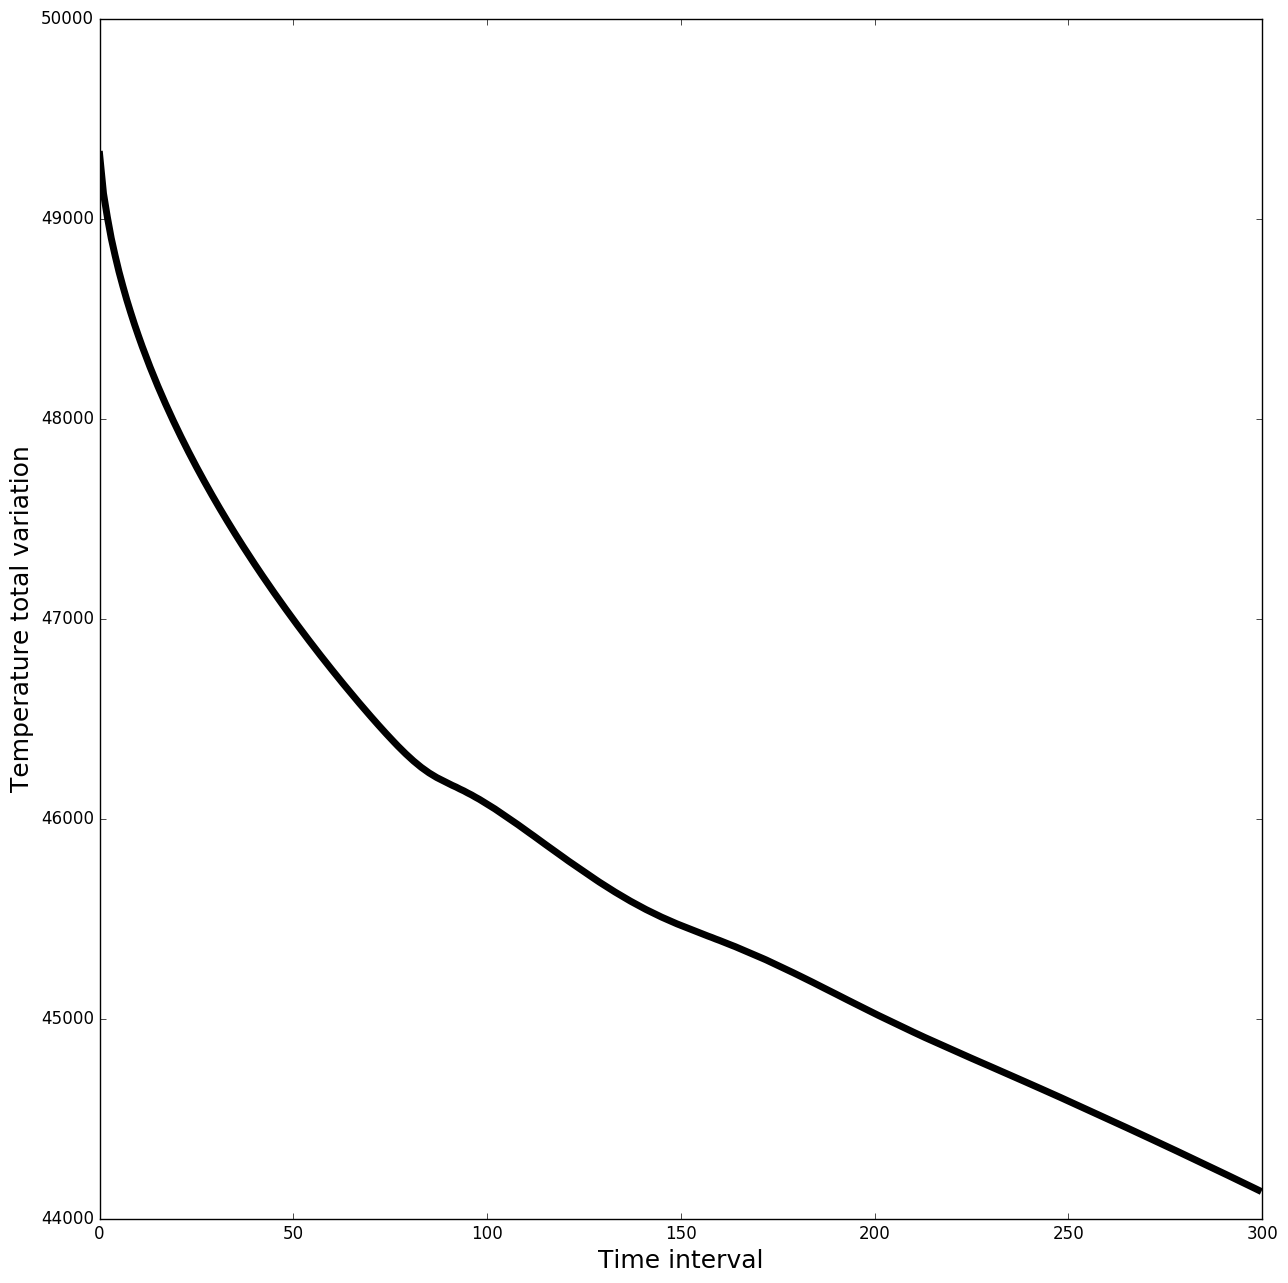
\includegraphics[width=0.5\textwidth]{../plots/tv-03.png}

    \justify
    \footnotesize{
    Figure 6: Temperature total variation (with respect to $T_{\mathrm{faucet}}$
    and with respect to the mean bathtub temperature over time in the case of a
    nonstationary fluid, with the same parameters as in Figure 5. The TV
    functions are considerably less well behaved, but notably the TV with
    respect to $T_{\mathrm{faucet}}$ decreases to a lower level than the same TV
in Figure 2.}
\end{center}

There are three interesting phenomena present in this result. First, we see that
the evolution of the total variation over time is less well-behaved than before.
We also note that the total variation with respect to the mean bathtub
temperature grows almost linearly with time and exhibits much less concavity
than Figure 2. Finally, the total variation with respect to
$T_{\mathrm{faucet}}$ reaches a lower threshold than the total variation in the
diffusion case only in Figure 2.

The choice of $b=5$ is essntially arbitrary; however the behavior of the fluid
with respect to different choices is highly volatile. In fact, modest changes to
the value for $b$ have drastic implications for the numerical stability of the
fluid flow, and consequently the temperature. We see this phenomenon in Figures
7 and 8. 

\begin{center}
    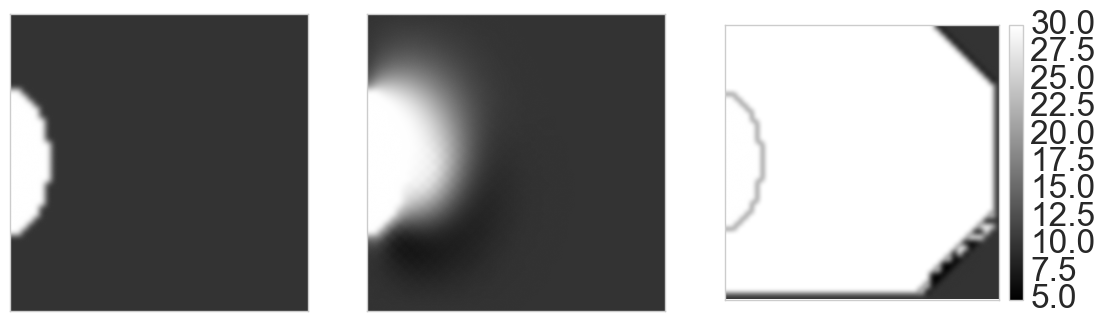
\includegraphics[width=0.8\textwidth]{../plots/diffusion-04.png}

    \justify
    \footnotesize{
    Figure 7: The heat diffusion process in the case of a moving fluid and
    permanent faucet tap. The mesh dimensions are $50 \times 50$, $\alpha =
    10^{-3}$, $T_{\mathrm{tub}} = 10$, and $T_{\mathrm{faucet}} = 30$. The
    parameter controlling the fluid motion is set $b = 8$. The numerical
    instability of the simulation causes the complete whitewashing by the final
frame.}
\end{center}

The evolution of frames in Figure 7 represents an explosion in the numerical
values associated with the temperatures. The black-white ridge in the bottom
right corner of the third frame exhibits the typical instability phenomenon we
observed in the simulations. Emanating from near the faucet source, this
phenomenon appears to push out towards the boundary of the frame until the
entire frame is whitewashed. We can also see this last-minute explosion by
measuring the total variation.

\begin{center}
    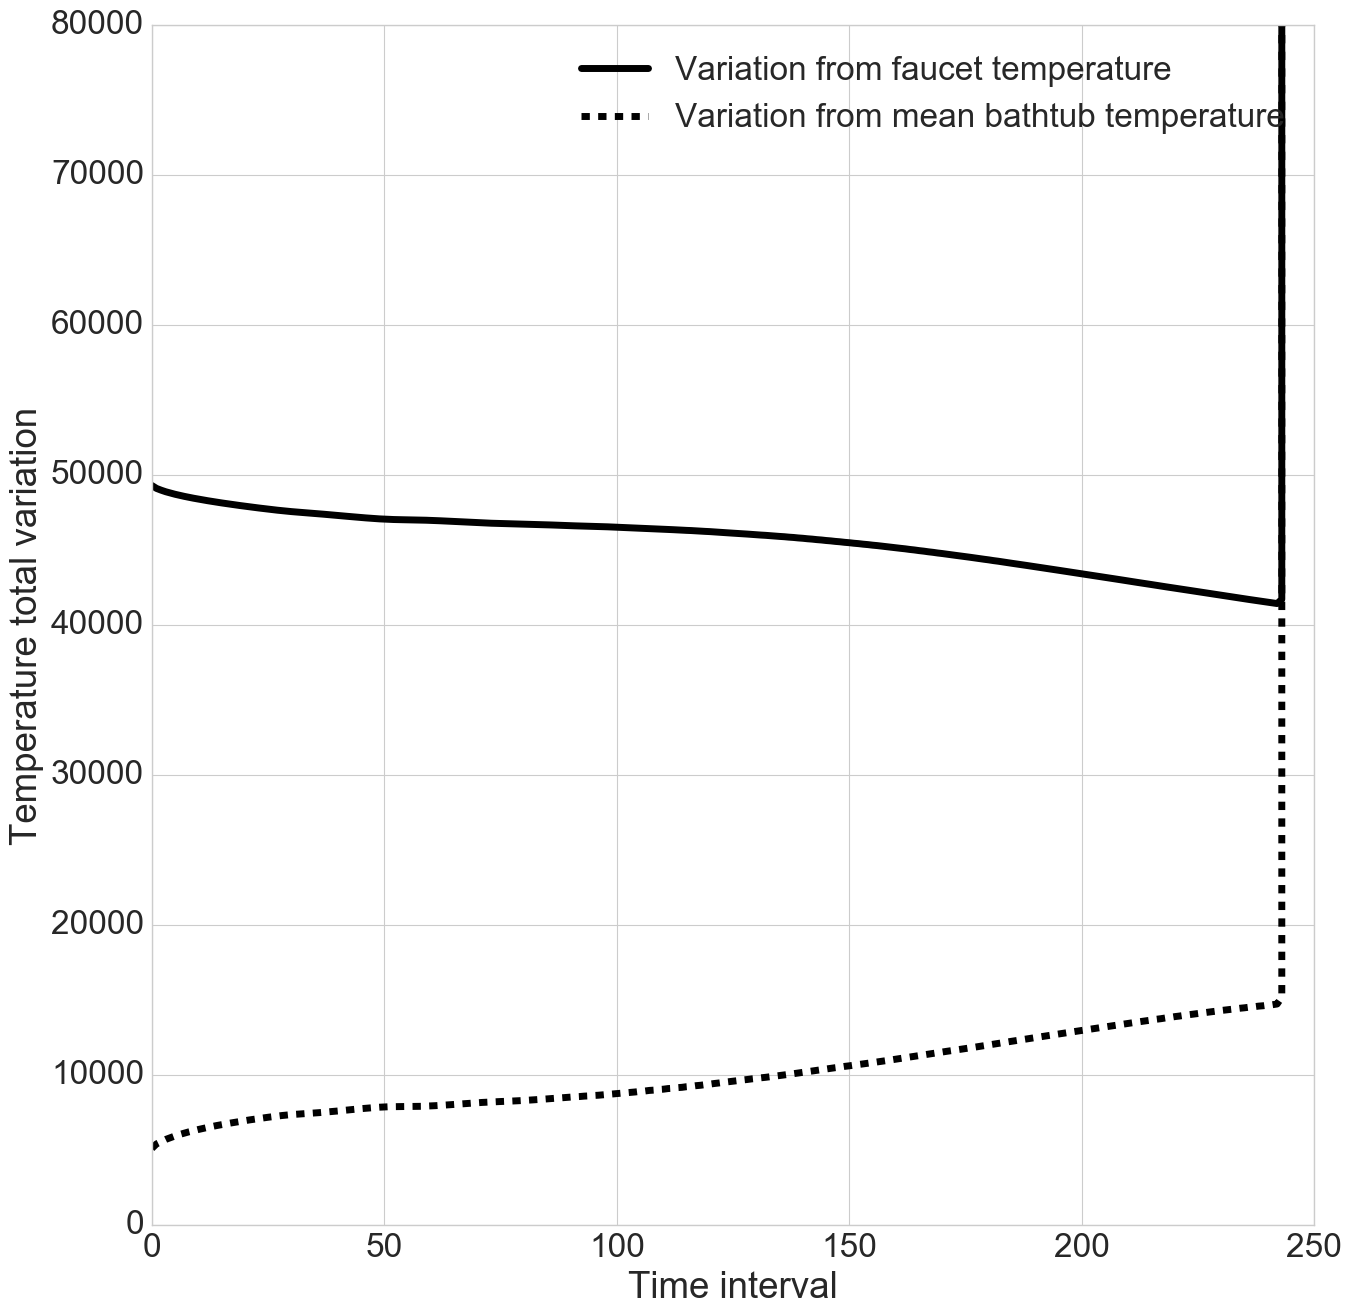
\includegraphics[width=0.5\textwidth]{../plots/tv-04.png}

    \justify
    \footnotesize{
    Figure 8: Temperature total variation (with respect to $T_{\mathrm{faucet}}$
    and with respect to the mean bathtub temperature over time in the case of a
    nonstationary fluid, with the same parameters as in Figure 5. The TV
    functions are considerably less well behaved, but notably the TV with
    respect to $T_{\mathrm{faucet}}$ decreases to a lower level than the same TV
in Figure 2.}
\end{center}

The presence of a constant heat and flow source in the faucet might suggest that
the numerical instability associated with the parametrization of $b$ relates
also to the source. We see that this is not the case. The numerical instability
persists even when the faucet is turned off, as in Figure 3.

\begin{center}
    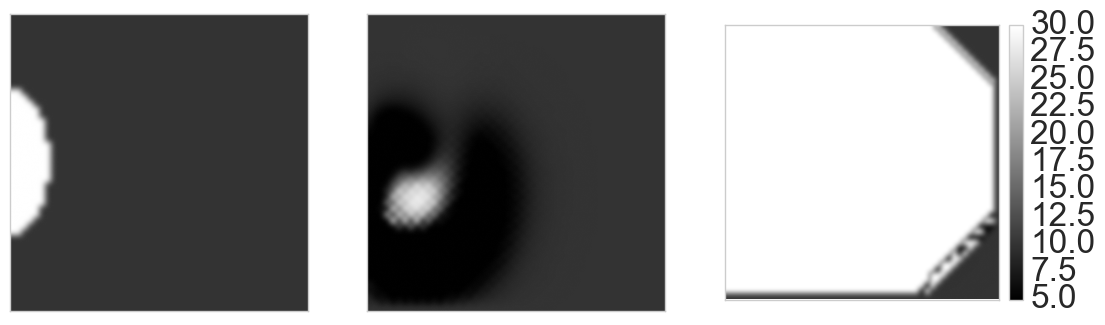
\includegraphics[width=0.8\textwidth]{../plots/diffusion-05.png}

    \justify
    \footnotesize{Figure 9: The heat diffusion process in the case of a moving fluid and
    temporary faucet tap. The mesh dimensions are $50 \times 50$, $\alpha =
    10^{-3}$, $T_{\mathrm{tub}} = 10$, and $T_{\mathrm{faucet}} = 30$. The
    parameter controlling the fluid motion is set $b = 8$. The numerical
    instability of the simulation causes the complete whitewashing by the final
frame.}
\end{center}

Interestingly, the second frame seems to show numerical instability towards
underflow, but by the third frame we observe near complete whitewashing of the
same characterization as Figure 7. We also see the black-white ridge in the
bottom right corner of the third frame, again in a similar fashion to Figure 7.

More surprisingly is the behavior of the temperature total variation, as we see
below in Figure 10.
\begin{center}
    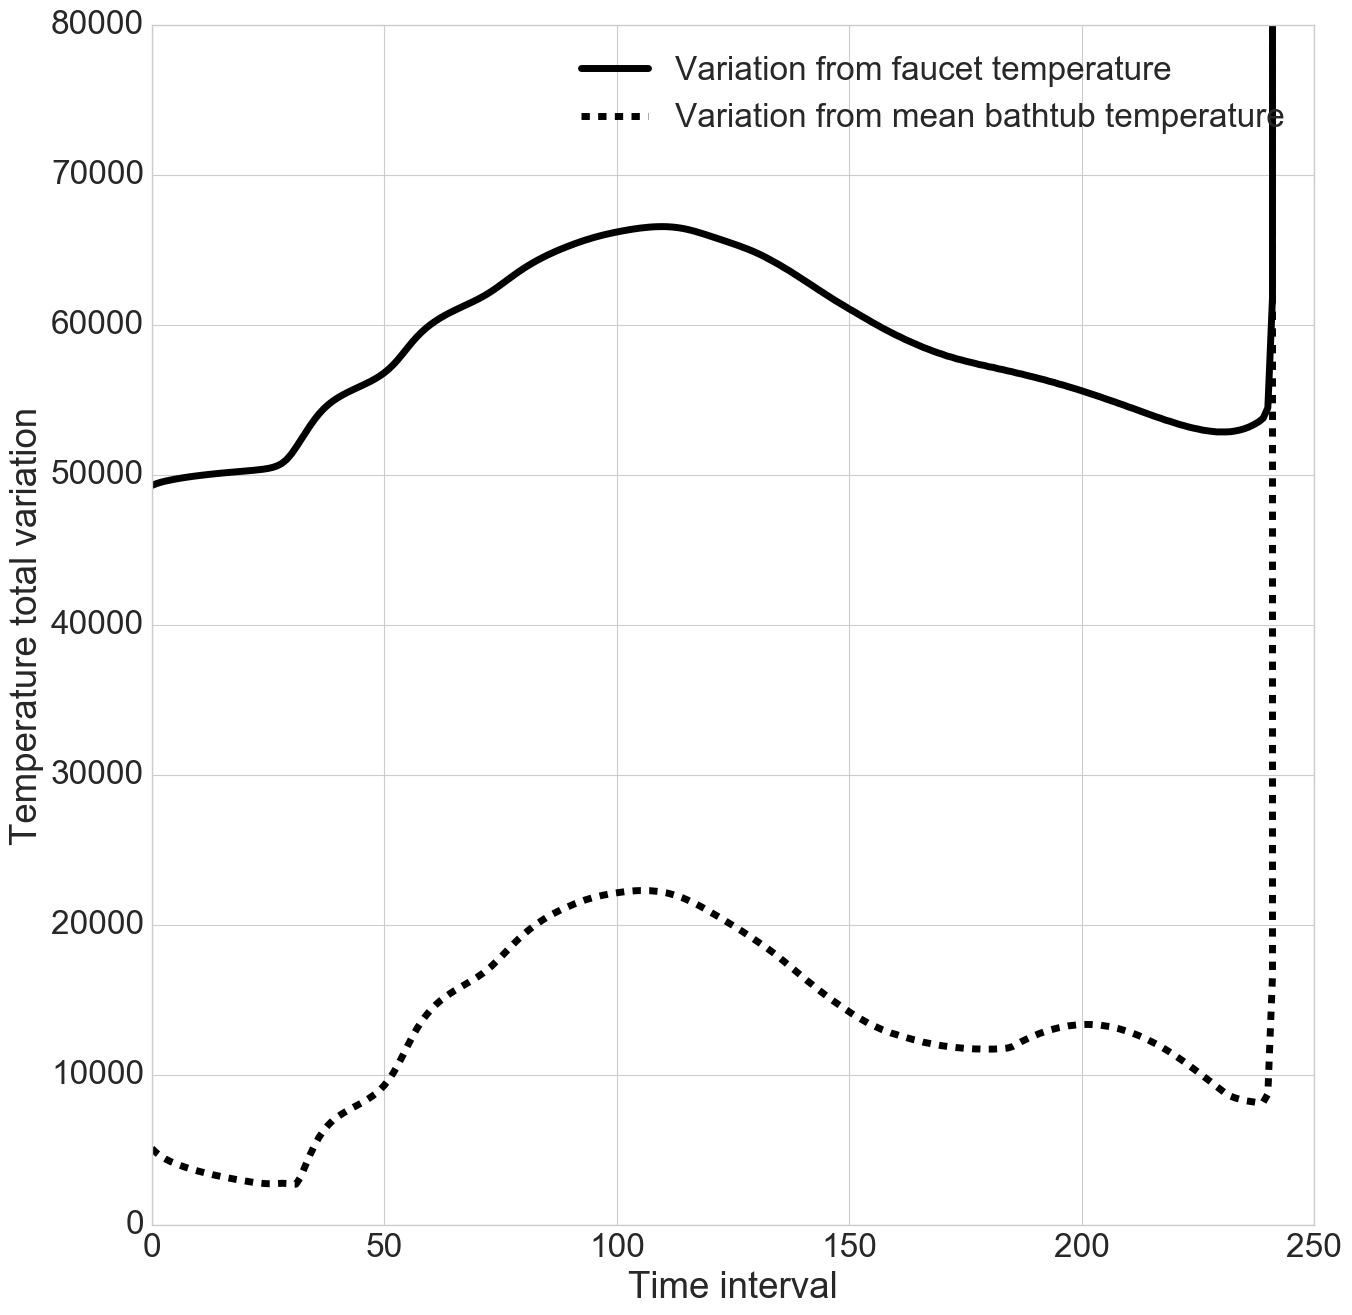
\includegraphics[width=0.5\textwidth]{../plots/tv-05.png}

    \justify
    \footnotesize{
        Figure 10: Temperature total variation (with respect to
        $T_{\mathrm{faucet}}$ and with respect to the mean bathtub temperature
        over time in the case of a nonstationary fluid, with the same parameters
        as in Figure 9. The TV functions are very poorly behaved and exhibit no
        similar characteristics to the previous configurations of the
        simulation.}
\end{center}
We have no intuition or explanation for the behavior of these total variation
functions. We suspect that this is almost entirely due to numerical artifacts in
the simulation but cannot speak with any authority to why the hump shape appears
in the plots. We do note, however, that the hump appears to correspond to the
second frame of Figure 9, in which we observe a very dark region with low
temperature. 




\section{Discussion}

As we showed in the previous section, our current numerical implementation of
the Navier-Stokes equations are highly sensitive to the initial conditions of
the model. Though a careful calibration of the deep parameters (e.g. $\rho$,
$\alpha$, $b$, etc.) and mesh granularity might produce more stable results,
we doubt that this would be sufficient. Fundamentally, forward Euler
approximations of the solutions to differential equations encourage volatility 
by accumulating the relatively small errors from the individual step
calculations into catastrophically unstable general results. To prevent this
kind of instability requires a re-examination of the numerical approach to
approximating these PDEs.

Perhaps somewhat surprising, then, is the fact that diffusion alone seems to
abstain from these stability problems. Indeed, if numerical differentiation is
the problem, then diffusion, which computes the Laplacian, should produce even
greater error. However, due to the simplicity of the stability conditions for
diffusion (for example, see Barba's discussion \cite{12-steps}), the checks on
stability can be readily accounted for and poor configuration choices can simply
be avoided. This was the approach of the study. From a cursory glance at the
Navier-Stokes and Poisson equations we understand that the stability conditions
are not necessarily so simple, but incorporating them should help improve the
reliability of the model.

That maintaining an active source (in the case of the bathtub narrative, a
running faucet) reduces the total variation of the temperature in the bathtub
supports our formulation of the optimization problem and also indicates suitable
choices for $\gamma$. Since including nonstationarity reduces the total
variation of the temperature the farthest, we can suggest to the avid bather
that keeping the water moving in the bathtub likely keeps the bathtub
temperature more evenly distributed than letting the water approach
stationarity.

Further investigation should attempt to mitigate the detrimental effects of
unchecked numerical instability. The mesh approach to the numerical
approximation of PDE solutions can be optimized \cite{betounes, 12-steps} to
minimize the accumulation of error. Solving our proposed optimization problem
requires additional study, too. Ultimately, our avid bather needs a policy to
maximize her utility, so specifying the ideal velocity $c$ remains the future
priority.

\nocite{*}


\printbibliography

\end{document}
